\documentclass[compress]{beamer}

\usetheme{Hamburg}

\usepackage[utf8]{inputenc}
%\usepackage{units}
\usepackage{algorithm}
\usepackage{algpseudocode}

\title{NeuGenGo}
\subtitle{Kann unser neuronales Netz besser Go spielen als wir?}
\author{Lennart Braun, Armin Schaare, Theresa Eimer}
\institute{Praktikum Parallele Programmierung \\Fachbereich Informatik\\Universität Hamburg}
\date{03.06.2015}

\begin{document}

\begin{frame}
	\titlepage
\end{frame}

\begin{frame}
	\frametitle{Gliederung (Agenda)}

	\tableofcontents
\end{frame}

\section{Ziele}

\begin{frame}
	\frametitle{Ziele}
	
	\begin{itemize}
		\item Ein gut spielendes Netz als Ergebnis
		\item Spiele und Netze visualisierbar machen
		\item Einen guten Vererbungsmechanismus finden
	\end{itemize}
	
\end{frame}

\section{Go}

\begin{frame}
	\frametitle{Go - Das Spiel}

	\begin{itemize}
		\item Asiatisches Brettspiel
		\item Wird auf Brettern mit 19x19 Knoten gespielt
		\item Ziel: gleichzeitig Gebiet einkreisen und gegnerische Steine schlagen
		\item Spielende: wenn beide Spieler passen
	\end{itemize}

	\begin{figure}
		\begin{center}
			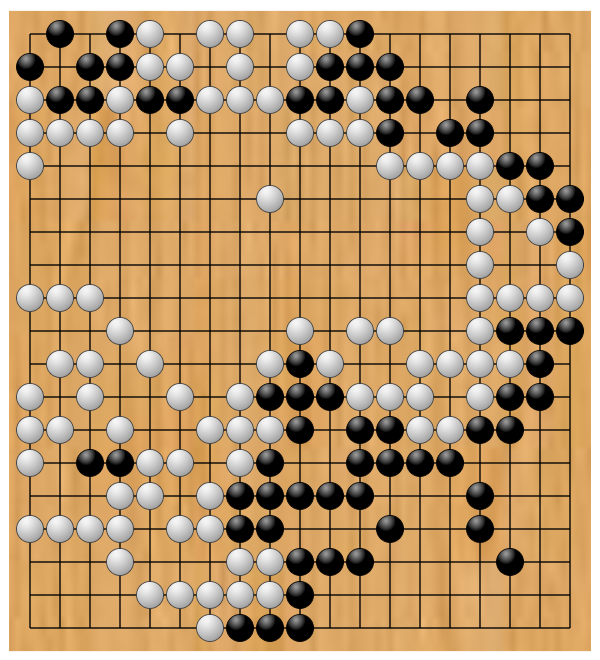
\includegraphics[scale=0.15]{board.png}
		\end{center}
		\caption{Beispiel eines Bretts}
		\begin{footnotesize}		 
		Quelle: http://www.13thmonkey.org/Artdraw/images/kifu2.png
		\end{footnotesize}
		\label{fig:Brett}
	\end{figure}
\end{frame}

\begin{frame}
	\frametitle{Go - Die Umsetzung}
	
	\begin{itemize}
		\item Gespielt wird auf kleineren Brettern (bis 9x9)
		\item Repräsentation des Brettes als eigener Datentyp, der den Spielzustand speichert
		\item Das Spiel endet, wenn es keine gültigen Züge mehr gibt
		\item Das Netz gibt pro Knoten eine Präferenz an, auf die höchste wird gesetzt
		\item Bei ungültigen Zügen wird die nächste Präferenz gezogen und es gibt einen Punktemalus. 
	\end{itemize}		
	
\end{frame}

\section{Das Netz}

\begin{frame}[fragile]
	\frametitle{Das Netz}

	\begin{itemize}
		\item Neuronales Netz mit...

		\begin{itemize}
			\item ...n+1 Input-Neuronen für n Knoten auf dem Spielfeld
			\item ...beliebig vielen hidden layers mit jeweils beliebig vielen Knoten
			\item ...2 Output-Neuronen für die x- bzw. y-Koordinate des nächsten Zuges (oder -1 / -1 zum Passen)
		\end{itemize}

		\item Ein Neuron gibt sein Signal weiter, wenn das aufsummierte Signal der Neuronen aus der Schicht davor einen festgelegten Wert übersteigt
	\end{itemize}
\end{frame}

\begin{frame}
	\frametitle{Was das Netz kann}
	
	\begin{itemize}
		\item Die Eingangssignale für die nächste Schicht an Neuronen berechnen
		\item Die Signale zu einer gültigen Ausgabe auswerten
		\item Den Aufbau des Netzes ausgeben
		\item Ein Netz als Datei ausgeben
		\item Mit dem Backpropagation Algorithmus supervised learning betreiben
	\end{itemize}
	
	\begin{figure}
		\begin{center}
			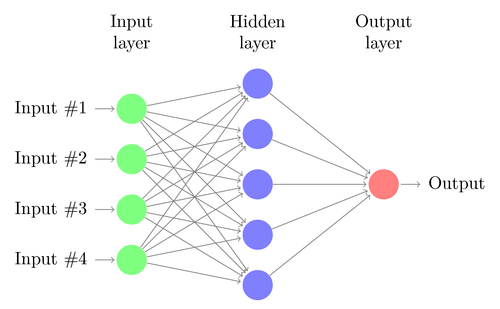
\includegraphics[scale=0.25]{net.png}
		\end{center}
		\caption{Beispielnetz}
		\begin{footnotesize}
		Quelle: http://www.texample.net/media/tikz/examples/PNG/neural-network.png
		\end{footnotesize}
		\label{fig:Netz}
	\end{figure}
	
\end{frame}

\section{Das Lernen}
\begin{frame}
	\frametitle{Lernen mit Backpropagation}
	
	\begin{itemize}
		\item Supervised learning mit Eingabedaten und erwarteten Werten
		\item Trainiert wird auf regelkonforme Züge
		\item Ziel: Präferenz für falsche Züge soll 0 sein
		\item Vergleich von Ausgabe und erwarteten Werten
		\item Gemäß dem Fehler werden die Kantengewichte von hinten nach vorne angepasst
	\end{itemize}
\end{frame}

\begin{frame}
	\frametitle{Der genetische Algorithmus}

	\begin{itemize}
		\item Je mehr Spiele ein Netz gewinnt, desto wahrscheinlicher überleben dessen Eigenschaften
		\item Verschiedene Möglichkeiten die Vererbung zu gestalten:

		\begin{itemize}
			\item Variable Lebensdauer von Netzen
			\item Verschiedene Mutationswahrscheinlichkeiten
			\item Crossovers
		\end{itemize}
		
		\item Finden der besten Kombination durch Ausprobieren
	\end{itemize}
\end{frame}

\section{Lösungsansatz}
\begin{frame}
    \frametitle{Lösungsansatz}

    Sequentieller Algorithmus
    \begin{algorithm}[H]
        \begin{algorithmic}[1]
            \State Generiere ein zufällige Menge $N_0$ an neuronalen Netzwerken
            \State Trainiere sie mit Backpropagation damit sie regelgerecht spielen
            \For {Runde $i = 0$ bis $\ldots$}
                \For {$n, m \in N_i$}
                    \State lass die Netze $n, m$ gegeneinander spielen
                    \State und zähle die Anzahl der Siege
                \EndFor
                \State generiere die Menge $N_{i+1}$ mit Hilfe eines genetischen
                Algorithmus abhängig von $N_i$ und den Ergebnissen der Spiele
            \EndFor
            \State Speichere die Netze
        \end{algorithmic}
    \end{algorithm}
\end{frame}
\begin{frame}
    \frametitle{I/O und Visualisierung}

    I/O
    \begin{itemize}
        \item Smart Game Format
            \begin{itemize}
                \item Speichern und Analyse von Partien
                \item Generieren von Trainingsdaten für die Netze
            \end{itemize}
        \item Go Text Protocol
            \begin{itemize}
                \item Kommunikation mit anderer Software
            \end{itemize}
        \item Dumps der neuronalen Netze
    \end{itemize}
    
    \hfill \\
    Visualisierung
    \begin{itemize}
        \item Abspielen von im SGF gespeicherten Partien
    \end{itemize}

\end{frame}

\section{Parallelisierungsschema}
\begin{frame}
    \frametitle{Parallelisierungsschema}

    Hybride Parallelisierung
    \begin{itemize}
        \item verteilter Speicher
            \begin{itemize}
                \item mehrere Partien auf verschiedenen Knoten
                \item Backpropagation auf verschiedenen Knoten
            \end{itemize}
        \item gemeinsamer Speicher
            \begin{itemize}
                \item parallele Berechnung der Ausgaben der neuronalen Netze
                \item ggf. Parallelisierung innerhalb des Go Moduls
            \end{itemize}
    \end{itemize}
\end{frame}

\end{document}
